\documentclass{article}
% --- watermark (auto-inserted) ---
\usepackage{xcolor}
\usepackage{xfp}% \fpeval; in the kernel since 2022, harmless on older LaTeX
\usepackage{draftwatermark}
\newlength{\watermarkTextWidth}
\AddToHook{begindocument/end}{%
  \SetWatermarkText{\normalfont Generated by The Agentic Scientist}%
  \SetWatermarkFontSize{10pt}%
  \SetWatermarkLightness{0.85}%
  \settowidth{\watermarkTextWidth}{\normalfont\fontsize{10pt}{12pt}\selectfont Generated by The Agentic Scientist}%
  \edef\watermarkScale{\fpeval{0.8 * sqrt(\paperwidth**2 + \paperheight**2) / \watermarkTextWidth}}%
  \edef\watermarkAngle{\fpeval{atand(\paperheight/\paperwidth)}}%
  \SetWatermarkScale{\watermarkScale}%
  \SetWatermarkAngle{\watermarkAngle}%
}
% --- end watermark ---
 % For LaTeX2e
\usepackage{paper,times}

\usepackage{hyperref}
\usepackage{url}
\usepackage{amsmath,amssymb}
\usepackage{graphicx}
\usepackage{booktabs}
\usepackage{subcaption}

\newcommand{\ts}{\boldsymbol{\theta}}
\newcommand{\sig}{\sigma}

\title{How Few Edits Displace the Top of a Bradley--Terry Leaderboard? A Verified First-Order Influence Probe on Crowd, Expert, LLM-Judge and Sports Comparison Data}
\author{Anonymous authors}

\begin{document}
\maketitle

\begin{abstract}
Pairwise-comparison leaderboards rank competitors by fitting a Bradley--Terry model to many ``A versus B'' judgments, yet it is unclear how few comparisons must change before the top-ranked competitor loses its place, and whether this differs between evaluation designs.
We measure this for a ridge-penalised Bradley--Terry fit, a single target (the rank-1 competitor), two edit modes (dropping rows or reversing outcomes) and budgets from 0.1\% to 2\% of rows.
Edits are proposed by a one-shot first-order influence search and scored by a trusted evaluator that refits the model on the edited data.
On held-out data from four designs (crowd votes, expert human judgments, LLM-judge judgments, basketball results) the family-averaged edit success score is 0.606, with per-design scores of 1.000, 0.833, 0.374 and 0.216, respectively.
At the 2\% budget the search displaces rank 1 in every crowd and sports case, in no LLM-judge case, and for expert human data only by reversing outcomes.
A simple win-rate heuristic scores 0.574.
These are bounded measurements of one heuristic attack on one target; they carry no sampling uncertainty, and the cause of the design ordering is untested.
\end{abstract}

\section{Introduction}
Public model-evaluation leaderboards often aggregate a large number of pairwise judgments (which of two responses, models or teams was better) into a Bradley--Terry (BT) score for every competitor, and then publish a ranking \citep{Bradley1952Rank,Chiang2024Chatbot}.
These rankings guide model selection, release announcements and research comparisons, so their dependence on the underlying comparison data matters.
Two lines of concern motivate this paper.
First, data are noisy and finite, so a small difference between the top two competitors may not be reliable \citep{Gao2021UncertaintyQI}.
Second, crowd-sourced leaderboards can be influenced deliberately: work on vote rigging on Chatbot Arena \citep{Min2025Rigging} and on the reliability of leaderboard rankings \citep{Singh2025Illusion} is motivation here (we know these two works from their titles only).
Both concerns lead to the same operational question: \emph{how many comparison rows have to be edited before the top-ranked competitor is no longer ranked first?}

We study this question for a deliberately narrow, fully specified setting.
The leaderboard is a ridge-penalised BT fit; the target is the competitor ranked first on the unedited data; an edit either drops a row or reverses its outcome; and the edit budget is between 0.1\% and 2\% of the rows.
A trusted evaluator, which never uses any quantity reported by the proposer, refits the model on the edited data and records whether rank 1 was displaced or, if not, what fraction of the top-versus-runner-up gap was closed.
The edits themselves are proposed by a one-shot first-order influence search in the spirit of influence functions \citep{Koh2017Understanding} and work on whether ``dropping a little data'' can change a conclusion \citep{Broderick2020Automatic} (known to us from its title only).
We apply it to held-out data from four evaluation designs that differ in who judges and what is judged: crowd-sourced human votes on chatbot responses \citep{Chiang2024Chatbot}, expert human judgments and GPT-4 judgments, both derived from the MT-Bench human-judgment dataset release \citep{Zheng2023Judging}, and National Basketball Association (NBA) game results.
Figure~\ref{fig:overview} summarises the protocol.

\begin{figure}[t]
\centering
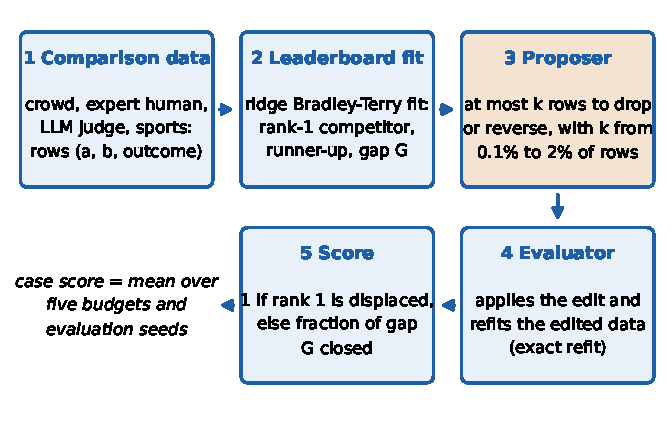
\includegraphics[width=0.95\textwidth]{figures/overview_protocol.pdf}
\caption{Evaluation protocol. Comparison rows from four evaluation designs are fitted with a ridge Bradley--Terry model, which fixes the rank-1 competitor and its gap $G$ to the runner-up. A proposer returns at most $k$ rows to drop or reverse, with $k$ from 0.1\% to 2\% of the rows. The evaluator refits the edited data, reports whether rank 1 changed, and otherwise reports the fraction of the gap closed.}
\label{fig:overview}
\end{figure}

\paragraph{What this paper is and is not.}
The studied search is the standard first-order influence heuristic, not a new algorithm, and we do not claim an improvement over any baseline: the evaluator's own influence baseline uses the same first-order formulas and obtains the same family-averaged score ($0.606$) as the studied search, so the margin over the best reference policy is exactly zero (Section~\ref{sec:results}).
Three alternative search variants were designed but produced no scored evidence and therefore support no comparison (Appendix~\ref{app:selection}).
The contribution is a controlled, verified measurement of how a fixed adversarial probe fares on four evaluation designs, together with a careful statement of what that measurement does and does not show.
Concretely:
\begin{itemize}
\item We specify an operational, evaluator-verified protocol (exact refit, five budgets, two edit modes, one target) that makes rank-1 vulnerability comparable across designs, and we derive the first-order effect of dropping or reversing a row, including an identity relating the two modes (Section~\ref{sec:method}).
\item We report that the probe's success is strongly design dependent: edit success scores of 1.000 (crowd), 0.833 (sports), 0.374 (expert human) and 0.216 (LLM judge), and 2\%-budget displacement in all crowd and sports cases but in no LLM-judge case (Section~\ref{sec:results}).
\item We document the validity checks that were run and the uncertainty that is unavailable, and we separate what the numbers show from hypotheses about the cause of the ordering, none of which was tested (Sections~\ref{sec:analysis} and~\ref{sec:limits}).
\end{itemize}

\section{Related Work}
\paragraph{Bradley--Terry models and their estimation.}
The BT model \citep{Bradley1952Rank} assigns each competitor a latent score and models the win probability of a pair as a logistic function of the score difference. Related work, which we know from titles only, includes BT models with ties \citep{Davidson1970OnET}, within-pair order effects \citep{Davidson1977OnET}, covariates \citep{Yan2025InferenceIA}, a dynamic BT model \citep{Tian2023ASA}, continuous data \citep{Stern2011ModeratedPC,Fageot2023GeneralizedBM} and a Bayesian approach \citep{Leonard1977AnAB}. Sports results are commonly rated with Elo-style systems that are closely related to BT-type likelihoods; recent work generalises Elo to the margin of victory \citep{Szczecinski2020GElo} and proposes a score-driven rating system for sports \citep{Holy2026ScoreDriven}. We fit a static BT model to NBA game outcomes only as a sports instance of pairwise-comparison data, and do not evaluate any Elo-style updating rule. Further titled works concern priorities from the BT model \citep{Genest1999DerivingPF}, its relation to PageRank \citep{Selby2024PageRankAT}, existence of maximum likelihood estimates \citep{Butler2004TheEO,Bong2021GeneralizedRF}, ridge regression for paired comparisons \citep{Varin2024TractableRR}, convergence rates of fitting algorithms \citep{Vojnovic2019ConvergenceRO}, and asymptotics of the BT model \citep{Simons1999AsymptoticsWT,Li2021ThePO}. We do not rely on any result from these works; our evaluator uses a ridge penalty and counts a tie as half a win for each side.

\paragraph{Uncertainty of rankings.}
Statistical work quantifies how sampling noise affects BT scores and ranks, through confidence regions for the score vector \citep{Gao2021UncertaintyQI}, hypothesis tests \citep{Makur2024MinimaxHT} and estimators of partial rankings from sparse, noisy comparisons \citep{Morel-Balbi2025EstimationOP}. These analyses describe average-case sampling variation under a generative model. We instead ask a worst-case, data-conditional question about a single observed dataset: whether a small number of specific rows can change the top rank. The two views are complementary, and our measurements do not substitute for either confidence intervals or noise calibration.

\paragraph{Influence and robustness to dropping data.}
Influence functions estimate the effect of removing or perturbing a training point without refitting \citep{Koh2017Understanding}. \citet{Broderick2020Automatic}, known to us from the title ``When Can Dropping a Little Data Make a Big Difference?'' only, ask whether dropping a small fraction of the data can change a conclusion. Our search shares the idea of choosing rows to drop by a first-order score, specialised to the top-versus-runner-up score gap of a BT fit and extended to outcome reversal, but we do not claim to reproduce their method. Linear approximations of this kind are related to the infinitesimal jackknife (\citealp{Giordano2018Swiss}, known to us from the title only); we rely on no accuracy guarantee, and the approximation may be inaccurate for the 2\% edits studied here. Because a first-order search finds candidate edit sets only, the evaluator verifies every edit by an exact refit.

\paragraph{Data poisoning and label-flip attacks.}
Choosing a small set of training points to manipulate so as to change a fitted model is the subject of data-poisoning research; influence-based reasoning has also been used on the defensive side, against poisoning in online learning \citep{Seetharaman2021Influence}. For preference data, \citet{Yang2026Preference} present a preference-poisoning attack on offline reinforcement learning from human feedback. We know these two works only from their titles and describe them no further. Our reversal mode is a label-flip edit and our drop mode a deletion, and the first-order scores in Eq.~\eqref{eq:effects} are likewise additive per row. The setting differs: the model is a Bradley--Terry leaderboard rather than a preference-optimised language model, the objective is to dislodge one rank rather than to steer parameters towards a target, and an evaluator refits the exact model for verification. We cite this literature for positioning only and do not compare against any poisoning method, and we have not surveyed attacks on rank aggregation exhaustively.

\paragraph{Integrity of crowd-sourced leaderboards.}
\citet{Chiang2024Chatbot} describe the Chatbot Arena platform, in which users vote between two anonymous model responses and the votes are aggregated into rankings. \citet{Min2025Rigging} (``Improving Your Model Ranking on Chatbot Arena by Vote Rigging'') and \citet{Singh2025Illusion} (``The Leaderboard Illusion'') concern the integrity of such leaderboards; we know both from their titles only and do not describe their methods or findings. \citet{Zheng2023Judging} release expert human and GPT-4 pairwise judgments on MT-Bench. We use the Arena and MT-Bench comparison data, but our attack is a generic, evaluator-verified probe; we do not model any platform's actual voting interface or an adversary's access to it.

\section{Problem Setting and Method}
\label{sec:method}
\subsection{Leaderboard, target and edit modes}
A comparison dataset is a list of $n$ rows $(a_i,b_i,y_i)$ over $K$ competitors, with $y_i\in\{+1,-1,0\}$ meaning that $a_i$ wins, $b_i$ wins, or the pair tied. Write $\tilde y_i\in\{1,\tfrac12,0\}$ for the corresponding win score of $a_i$. The evaluator fits $\ts\in\mathbb{R}^K$ by maximising the penalised log-likelihood
\begin{equation}
\ell(\ts)=\sum_{i=1}^{n}\Big[\tilde y_i\log\sig(\theta_{a_i}-\theta_{b_i})+(1-\tilde y_i)\log\sig(\theta_{b_i}-\theta_{a_i})\Big]-\tfrac{\lambda}{2}\sum_{k}\theta_k^2,\qquad \lambda=10^{-3},
\label{eq:bt}
\end{equation}
to gradient tolerance $10^{-10}$. A tie therefore counts as half a win for each side. The rank-1 competitor is $\mathrm{top}=\arg\max_k\hat\theta_k$, the runner-up is $\mathrm{rv}=\arg\max_{k\neq \mathrm{top}}\hat\theta_k$, and the \emph{gap} is $G(\ts)=\theta_{\mathrm{top}}-\max_{j\neq \mathrm{top}}\theta_j$. % @evidence[[source_evidence/downstream/program/src/program.py#handle]]
The target is to make the unedited rank-1 competitor no longer rank first after the edit, that is, to drive $G$ below zero on the refit of the edited data.
There are two edit modes. In \emph{drop} mode, the chosen rows are removed. In \emph{flip} mode, the outcomes of the chosen rows are reversed, which is only allowed for decisive rows ($y_i\neq 0$). We call the second mode ``reversal'' in prose and use the evaluator's name ``flip'' only for the mode label, to avoid confusion with displacement rates.
The budget is $k=\max(1,\lceil fn\rceil)$ with $f\in\{0.1\%,0.25\%,0.5\%,1\%,2\%\}$ of the rows.\footnote{The five budget fractions are fixed in the evaluator's budget ladder.} % @evidence[[source_evidence/task/evaluate_final.py#LADDER]]
The proposer receives the raw arrays with anonymised competitor indices and returns at most $k$ distinct row indices; any malformed answer scores zero for that budget.

\subsection{First-order influence edit search}
\label{sec:influence}
The studied search fits $\hat\ts$ once, and then ranks rows by the first-order change of the gap that editing each row would cause. Let $p_i=\sig(\hat\theta_{a_i}-\hat\theta_{b_i})$ and let $A=\sum_i p_i(1-p_i)(e_{a_i}-e_{b_i})(e_{a_i}-e_{b_i})^{\top}+\lambda I$ be the negative Hessian of Eq.~\eqref{eq:bt}. The score gradient contributed by row $i$ is $(\tilde y_i-p_i)(e_{a_i}-e_{b_i})$. Removing the row perturbs the stationarity condition by $-(\tilde y_i-p_i)(e_{a_i}-e_{b_i})$, so a Newton step gives the parameter change $A^{-1}$ times that perturbation. Define the sensitivity direction and the row coefficient
\begin{equation}
v=A^{-1}(e_{\mathrm{top}}-e_{\mathrm{rv}}),\qquad s_i=v_{a_i}-v_{b_i}.
\end{equation}
The first-order change of the (top versus runner-up) gap is then
\begin{equation}
\Delta_i^{\mathrm{drop}}=-s_i\,(\tilde y_i-p_i),\qquad
\Delta_i^{\mathrm{flip}}=s_i\,(1-2\tilde y_i),
\label{eq:effects}
\end{equation}
where the second expression is the effect of replacing $\tilde y_i$ by $1-\tilde y_i$. The search returns the (at most) $k$ rows with the most negative $\Delta_i$ among admissible rows (all rows for drop, decisive rows for flip), discarding rows with $\Delta_i\ge 0$ and breaking ties by row index, so the output is deterministic. The implementation fits $\hat\ts$ by Newton iterations on the $K\times K$ pair-count matrix, then solves a single $K\times K$ linear system for $v$. % @evidence[[source_evidence/downstream/program/src/program.py#_propose]]

Three properties of Eq.~\eqref{eq:effects} shape how the results should be read.
\emph{(i) Additivity.} The per-row effects are summed without modelling how $p_i$ and $A$ change after many rows are edited, so the heuristic can be inaccurate at a 2\% budget even when it is accurate for one row; we did not evaluate the accuracy of the underlying linear approximation for these data.
\emph{(ii) A fixed rival.} The direction is built for the initial runner-up only. If an edit set raises a different competitor above the incumbent, the search does not anticipate it, although the evaluator would credit the displacement.
\emph{(iii) Flip versus drop.} Reversing a row is equivalent to dropping it and inserting the opposite outcome, so $\Delta^{\mathrm{flip}}_i=\Delta^{\mathrm{drop}}_i+s_i\,((1-\tilde y_i)-p_i)$. For a decisive row, $\tilde y_i-p_i$ has the sign of $\tilde y_i-\tfrac12$, so the two modes select gap-reducing rows by the same sign condition on $s_i$, and the flip effect is larger by the factor $1/|\tilde y_i-p_i|>1$. At first order, reversal is therefore the stronger edit for the same number of rows; this is a statement about Eq.~\eqref{eq:effects}, not an empirical finding.

\subsection{Scoring and verification}
For each budget level, the evaluator refits the edited data with its own damped-Newton fitter and ignores any quantity the proposer reports about gaps or ranks. The score of a level is $1$ if the original top competitor is no longer first, and otherwise $\mathrm{clip}(1-G_{\text{after}}/G_{\text{before}},0,1)$, the fraction of the gap that was closed. The \emph{edit success score} of a case is the mean over the five budgets and over evaluation seeds; the score of a design is the mean over its cases; and the \emph{family-averaged} edit success is the equally weighted ($0.25$ each) mean over the four designs. The \emph{top-1 displacement rate at the 2\% budget} of a design and mode is the mean of the displacement indicator at the largest budget over the cases and seeds in that cell. Invalid or missing answers count as worst case. % @evidence[[source_evidence/task/evaluate_final.py#aggregate]]

\subsection{Reference policies and controls}
Three evaluator-owned reference policies, which never contact the proposer, calibrate the scale of the scores. The \emph{constant} policy averages the score of an empty edit and of editing the first $k$ rows in file order. The \emph{random} policy averages 20 uniformly random edit sets of the same size. The \emph{win-rate heuristic} selects rows in which the incumbent top competitor won, preferring rows against the runner-up. The evaluator also computes its own first-order influence baseline with the same formulas as Section~\ref{sec:influence}. % @evidence[[source_evidence/task/evaluate_final.py#baseline_scores]]
A \emph{permuted-input control} re-runs the proposer on a row-shuffled, competitor-relabelled copy of each case, maps the proposed rows back to the original data and scores them with the same refit; the reported statistic is the mean absolute difference from the unpermuted score. The \emph{valid proposal rate} is the fraction of budget-level answers that passed format checks.

\subsection{Evaluation designs}
\label{sec:designs}
Table~\ref{tab:designs} lists the designs. Every design is evaluated in both edit modes, so crowd, expert-human and LLM-judge data contribute one case per mode, and sports data three NBA seasons per mode. The sealed final data are disjoint from the data used to choose the search configuration (verified by content hashes in the task protocol), and anonymised competitor indices carry no model or team names. For NBA games, the home team is listed first as $a_i$ purely as a row convention; the Bradley--Terry model of Eq.~\eqref{eq:bt} has no home-advantage term, whereas Elo-style sports ratings \citep{Szczecinski2020GElo,Holy2026ScoreDriven} are typically updated game by game, so our static fit is a simplification of how such ratings are produced. % @evidence[[source_evidence/task/task_contract.json#provenance]]

\begin{table}[t]
\centering
\caption{Evaluation designs of the sealed final evaluation. Cases are (data source $\times$ edit mode). Dataset sizes and competitor counts are not used in this paper.}
\label{tab:designs}
\small
\begin{tabular}{p{2.0cm}p{5.5cm}p{1.5cm}p{2.7cm}}
\toprule
Design & Data source & Cases & Competitors \\
\midrule
Crowd votes & Held-out partition of public Chatbot Arena human-preference votes \citep{Chiang2024Chatbot} & 2 (drop, flip) & Anonymised chatbots \\
Expert human & MT-Bench expert human pairwise judgments \citep{Zheng2023Judging}; ties kept & 2 & Anonymised models \\
LLM judge & GPT-4 pairwise judgments from the same dataset release; two tie labels mapped to a tie & 2 & Anonymised models \\
Sports & NBA regular-season games of 2008, 2012, 2015; home team listed first & 6 (3 seasons $\times$ 2) & Teams of one season \\
\bottomrule
\end{tabular}
\end{table}

\subsection{Experimental protocol and reporting}
The proposer is evaluated once on the sealed final data with three evaluation seeds (201, 202, 203). A seed only resets proposer state; it never selects data or workload. Because the proposer is deterministic, the three seeds are replicate executions of the same computation and carry no information about sampling variability of the data. Search-time scores were obtained on a separate proxy data collection (different Arena partition and NBA seasons, no expert-human or LLM-judge data, and an additional declared-synthetic planted near-tie family with weight 0.2 in the search-scope score) and are reported only as separate context in Appendix~\ref{app:selection}; they are never compared with the final scores.

\section{Results}
\label{sec:results}
All numbers in this section come from the sealed final evaluation, whose qualification outcome is \emph{qualified} with status \emph{completed}. % @evidence[[paper_data.json#final_evaluation.outcome]]
Qualification certifies that the run was complete and valid (full declared transcript, trusted-refit scoring, non-vacuous controls, all reference policies computed); it is not evidence of superiority or of generality. Candidate-reported diagnostics are marked unverified by the evaluator and are not used here. % @evidence[[paper_data.json#final_evaluation.evaluation_evidence.candidate_diagnostics_trust]]

\subsection{Edit success differs strongly across evaluation designs}
The family-averaged edit success score of the first-order influence search is $0.606$. % @evidence[[paper_data.json#final_evaluation.metrics.combined_score]]
Panel (a) of Figure~\ref{fig:scores} shows the per-design scores: crowd votes $1.000$, sports $0.833$, expert human $0.374$ and LLM judge $0.216$. % @evidence[[paper_data.json#final_evaluation.metrics.score_crowd]] @evidence[[paper_data.json#final_evaluation.metrics.score_sports]] @evidence[[paper_data.json#final_evaluation.metrics.score_expert_human]] @evidence[[paper_data.json#final_evaluation.metrics.score_llm_judge]]
Because a level scores at most one and exactly one only when rank 1 is displaced (up to an exact tie), a design score of $1.000$ means that rank 1 was displaced at every one of the five budgets, including the smallest (0.1\% of rows), in both crowd cases. The sports score of $0.833<1$ implies that at least one smaller budget in at least one sports case did not displace rank 1. For the LLM judge, rank 1 was not displaced at the 2\% budget in either mode (Table~\ref{tab:disp}), so the score of $0.216$ reflects partial closure of the gap.

\begin{figure}[t]
\centering
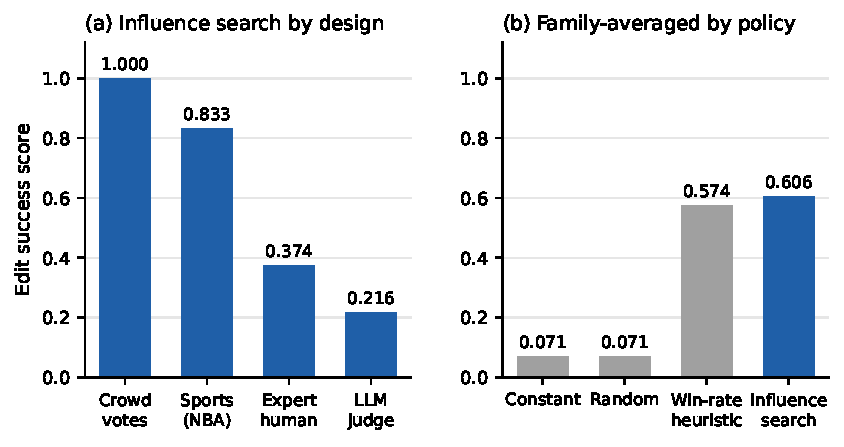
\includegraphics[width=\textwidth]{figures/design_scores.pdf}
\caption{Edit success score on the sealed final data (higher means rank 1 was displaced more reliably or a larger fraction of the gap was closed). (a) The first-order influence search for each evaluation design. (b) Family-averaged scores (equal weights over the four designs) for the evaluator's reference policies and the studied search; blue marks the studied search. Each bar is a single deterministic evaluation value; no uncertainty interval exists.}
\label{fig:scores}
\end{figure}

\subsection{Top-1 displacement at the largest budget}
Table~\ref{tab:disp} reports the displacement rate at the 2\% budget by design and edit mode. % @evidence[[paper_data.json#final_evaluation.metrics.flip_rate_crowd_drop]] @evidence[[paper_data.json#final_evaluation.metrics.flip_rate_expert_human_flip]]
Rank 1 is displaced in every crowd and sports case in both modes. For expert human data only reversal succeeds, and for the LLM judge neither mode does. Because each crowd, expert-human and LLM-judge cell contains a single case and the proposer is deterministic, every entry is $0$ or $1$; the sports entries average three seasons and also happen to be $0$ or $1$.
The ordering by edit success score (crowd, sports, expert human, LLM judge) is thus mirrored by the number of design--mode cells in which the heuristic reaches displacement at 2\% (2, 2, 1, 0 of 2).

\begin{table}[t]
\centering
\caption{Sealed final evaluation: per-design edit success score and top-1 displacement rate at the 2\% budget by edit mode. Entries in the displacement columns are the means over cases and seeds in the cell (one case for crowd, expert human and LLM judge; three seasons for sports).}
\label{tab:disp}
\small
\begin{tabular}{lcccc}
\toprule
Design & Cases & Edit success & Displaced at 2\%, drop & Displaced at 2\%, flip \\
\midrule
Crowd votes  & 2 & 1.000 & 1.0 & 1.0 \\ % @evidence[[paper_data.json#final_evaluation.metrics.flip_rate_crowd_flip]]
Sports       & 6 & 0.833 & 1.0 & 1.0 \\ % @evidence[[paper_data.json#final_evaluation.metrics.flip_rate_sports_drop]] @evidence[[paper_data.json#final_evaluation.metrics.flip_rate_sports_flip]]
Expert human & 2 & 0.374 & 0.0 & 1.0 \\ % @evidence[[paper_data.json#final_evaluation.metrics.flip_rate_expert_human_drop]]
LLM judge    & 2 & 0.216 & 0.0 & 0.0 \\ % @evidence[[paper_data.json#final_evaluation.metrics.flip_rate_llm_judge_drop]] @evidence[[paper_data.json#final_evaluation.metrics.flip_rate_llm_judge_flip]]
\midrule
Family average & 12 & 0.606 & \multicolumn{2}{c}{not defined} \\
\bottomrule
\end{tabular}
\end{table}

\subsection{Reference policies set the scale}
Panel (b) of Figure~\ref{fig:scores} compares the studied search with the evaluator's reference policies on the same family-averaged scale. The constant and random policies score $0.071$ each, so, averaged over all cases, a generic perturbation of at most 2\% of the rows closes only a small fraction of the gap. This suggests that the displacement obtained in crowd and sports data owes more to targeted row selection than to perturbation in general, although per-design values for the random policy are not available to check it. % @evidence[[paper_data.json#final_evaluation.metrics.score_constant]] @evidence[[paper_data.json#final_evaluation.metrics.score_random]]
The win-rate heuristic, which selects rows by the incumbent's wins, preferring those against the runner-up, scores $0.574$ against $0.606$ for the influence search, a difference of $0.032$. % @evidence[[paper_data.json#final_evaluation.metrics.score_winrate]] @evidence[[paper_data.json#final_evaluation.metrics.score_influence]]
This is one evaluation value per policy without an uncertainty estimate and without per-design values for the reference policies; we therefore make no claim about which of the two policies is better. The margin of the studied search over the best reference policy is $0.0$, because the evaluator's influence baseline, which uses the same first-order formulas, attains the same family-averaged score as the studied search (both $0.606$). The two procedures differ in detail (the studied search discards rows with non-negative first-order effect, whereas the evaluator's baseline filters only non-finite effects, and the baseline uses the evaluator's own fitter), and we did not compare their edit sets row by row. % @evidence[[paper_data.json#final_evaluation.metrics.margin_vs_best_baseline]]
The task protocol declares a separate claim of outperforming the reference policies, which requires a positive margin and a paired-bootstrap interval excluding zero; that claim is not met here. % @evidence[[source_evidence/task/task_contract.json#protocol.promotion_rule]]

\subsection{Validity checks and run-to-run behaviour}
The valid proposal rate is $1.0$: every answer to every budget level passed the format checks. The permuted-input control gap is $0.0$: on the single row-shuffled, relabelled control run per case, the proposer's scores matched its scores on the original order (mean absolute gap $0.0$). This is one permutation per case and does not establish invariance to row order or competitor labels in general. % @evidence[[paper_data.json#final_evaluation.metrics.valid_proposal_rate]] @evidence[[paper_data.json#final_evaluation.metrics.perm_control_abs_gap]]
The three evaluation seeds produce identical family-averaged scores ($0.6057$ each), as expected for a deterministic proposer on fixed data. % @evidence[[paper_data.json#final_evaluation.evaluation_evidence.episodes]]
This agreement should not be read as low variability of the leaderboard under resampling: no bootstrap, subsampling or noise model was applied to the data, so we report no confidence interval.

\section{What the Evidence Does and Does Not Show}
\label{sec:analysis}
\subsection{A measured ordering, not a general sensitivity law}
The measurement supports the statement that, with this heuristic, within these budgets and on these twelve cases, rank-1 vulnerability decreases in the order crowd, sports, expert human, LLM judge. The ordering is an observation for one attack and one target. Failure to displace rank 1 (LLM judge in both modes, expert-human data in drop mode) shows only that this one-shot first-order heuristic did not succeed within 2\% of the rows. It is not a certificate that no successful edit set exists, and a stronger search could close the gap in cells where this one did not. Conversely, success in crowd and sports data shows that rank 1 can be displaced with at most the budget used, not that it is the smallest such edit set.

\subsection{Candidate explanations, all untested}
The artifacts contain no experiment that connects the ordering to a mechanism. We list candidate explanations to guide follow-up work and label each as a hypothesis.
\begin{itemize}
\item \emph{Margin relative to data mass.} The relative size of the rank-1 gap compared with the total information in the data determines how many rows must move; designs with a thin top margin would be easier to dislodge. Gaps and row counts per design are not available to us, so this is unchecked.
\item \emph{Concentration of influence.} If the coefficients $s_i$ concentrate on few pairs (for example, matches between the top two competitors), few edits can matter; how concentrated they are depends on the comparison graph of each design, which we did not inspect.
\item \emph{Number of competitors and graph density.} The designs differ in the number of competitors in ways not measured here. Whether the number of competitors helps or hinders displacement is not established by four designs.
\item \emph{Tie handling.} Ties count as half a win and cannot be reversed in flip mode. Designs with many ties have fewer rows available for reversal; we did not tabulate tie fractions, so we cannot say whether this matters here.
\item \emph{Linearisation error.} A 2\% edit of a small dataset is a larger perturbation of $A$ and $p$ than a 2\% edit of a large one, so the additive first-order approximation may degrade differently across designs.
\end{itemize}
Designs are confounded: they differ at the same time in dataset size, number of competitors, rank-1 margin, tie rate and judge type, and each design has few cases. No single factor can be isolated from this experiment, and the sequentially tuned, single-configuration setup provides no ablations.

\subsection{Expert human versus GPT-4 judge}
The expert-human and GPT-4 designs are both derived from the MT-Bench human-judgment dataset release; the overlap of rows, questions and models between the two final row sets was not verified. For expert human data, reversal displaces rank 1 at 2\% while dropping does not; for GPT-4 judgments neither works, and the edit success score is lower ($0.216$ versus $0.374$). The cause is untested. Differences in the number of judgments, the fraction of ties (including the second tie label in the GPT-4 data), and the size of the rank-1 gap are all plausible, and each design has one case per mode, so this is a difference between two single measurements and not a statistical result about human versus LLM judges.

\subsection{Drop versus reversal}
In the one design where the two modes differ (expert human), reversal succeeds and dropping does not. This is consistent with property (iii) of Section~\ref{sec:influence}: for the same rows, reversal has a larger first-order effect than removal by the factor $1/|\tilde y_i-p_i|$. It remains a single-cell observation: in crowd and sports data both modes displace rank 1 and in LLM-judge data neither does, so the mode matters in only one of the four designs.

\subsection{What a stronger test of sensitivity would need}
Our results leave the original question (sensitivity to small changes from noise or from intent) only partly answered. Answering it would require, at least: edit-size curves for minimal displacing sets from a search with a verified lower-bound or certificate, not only a one-shot heuristic; noise calibration against resampled data (for example, comparing edit sizes with the sampling variability of the gap); several cases per design with confidence intervals; and ablations over subsample size and tie handling. None of these was performed here, and we state them as open rather than as completed work.

\section{Limitations}
\label{sec:limits}
\paragraph{One attack, one target.} Only a one-shot first-order search with a single rival direction at the initial fit is evaluated, and only the displacement of rank 1 is targeted. Other targets (top-$m$ sets, pairwise order of two chosen competitors) and iterative or batched searches are not covered.
\paragraph{Fixed leaderboard specification.} The evaluator's BT specification (ridge $10^{-3}$, tie as half a win) is part of the measurement. We do not know how conclusions change for other regularisation strengths, tie models or rating systems.
\paragraph{Design confounds and few cases.} The four designs are specific datasets, not random draws from design classes; they are confounded with size, number of competitors, margin and tie rate. Three of the four designs have one case per edit mode. The NBA data are game results, not preference or judge data, and serve as a sports proxy. Expert-human and LLM-judge data come from the same dataset release, but row-, question- and model-level overlap was not verified.
\paragraph{No sampling uncertainty and no noise-versus-intent attribution.} The identical seeds reflect determinism, and no resampling was performed; we therefore cannot say whether the observed vulnerability exceeds ordinary sampling variation of the leaderboard, nor whether it corresponds to plausible noise or to deliberate manipulation. We also do not model what an adversary could actually do on a real platform.
\paragraph{Missing diagnostics and aggregate-only baselines.} Per-case gaps, row counts, budget-level scores and per-design values for the reference policies were not available to the analysis, and the evaluator marks candidate diagnostics as unverified. The comparison with the win-rate heuristic is therefore a single aggregate difference.
\paragraph{No improved search.} Three alternative search designs were not scored (Appendix~\ref{app:selection}), so no statement about improved or minimal edit sets can be drawn.

\section{Conclusion}
We measured, with exact-refit verification, how a one-shot first-order influence search fares at displacing the rank-1 competitor of a ridge Bradley--Terry leaderboard using 0.1\% to 2\% of the rows, on crowd, expert-human, LLM-judge and sports data. The family-averaged edit success is 0.606, and it varies strongly by design: 1.000 for crowd votes, 0.833 for sports, 0.374 for expert human data and 0.216 for the LLM judge. At 2\% the heuristic displaces rank 1 in every crowd and sports case, never for the LLM judge, and for expert human data only by reversing outcomes. A win-rate heuristic reaches 0.574, a difference too small to rank the two policies without uncertainty estimates. Qualification of the evaluation attests to its validity, not to superiority or generality; the margin over the best reference policy is zero because the studied search is the evaluator's influence baseline.
The result is a bounded measurement for one probe, one target and four datasets. It shows that rank-1 vulnerability under this attack is highly heterogeneous across evaluation designs, which argues against reporting a single sensitivity number for leaderboards. It does not show why, does not separate noise from intent, and does not show minimal edit sizes. Resampling-based calibration, several cases per design and stronger searches are the natural next steps.

% IMPORTANT: \clearpage flushes all pending floats before references so that
% body-page counting excludes reference-only pages.  Do NOT remove.
\clearpage
\bibliography{references}
\bibliographystyle{paper}

\clearpage
\appendix
\section{Supplementary Information}

\subsection{Evaluator Specification and Metric Definitions}
\label{app:eval}
The evaluation interface is a request--response protocol with a reset operation (clearing all proposer state and seeding it) and a propose operation. Each propose request carries the mode, the budget $k$, the number of competitors, the number of rows and base64-encoded integer arrays of competitor indices and outcomes, with rows in the order of the original data. Each call has a hard wall-clock limit of 30 seconds, and the proposer runs on CPU with two threads. Responses with extra keys, non-integer or duplicate or out-of-range indices, more than $k$ indices, or tie rows in flip mode are invalid and score zero for that level. % @evidence[[source_evidence/downstream/program/src/program.py#handle]]
The sealed final evaluation has twelve cases (crowd, expert human and LLM judge: one data source $\times$ two modes; sports: three seasons $\times$ two modes), three primary seeds and one permuted control episode per case, with each episode issuing five budget calls. % @evidence[[source_evidence/task/evaluate_final.py#CASE_SPECS]]
Design scores average cases within a design; family weights are $0.25$ each. The evaluator computes ranks and gaps from its own Newton fit, and its Newton fitter was cross-checked once against an independent L-BFGS fit on at most the first 600 rows of the smallest case (not on every edited refit or unedited case); the target is judged on the original rank-1 competitor's gap to the best other competitor on the refit of the edited data.

\subsection{Complete Final Metric Table}
\label{app:metrics}
Table~\ref{tab:allmetrics} lists all retained sealed-final metrics.
\begin{table}[h]
\centering
\caption{All retained metrics of the sealed final evaluation (three evaluation seeds, identical across seeds). Displacement rates are at the 2\% budget.}
\label{tab:allmetrics}
\small
\begin{tabular}{lr}
\toprule
Metric & Value \\
\midrule
Family-averaged edit success (influence search) & 0.6057 \\ % @evidence[[paper_data.json#final_evaluation.metrics.combined_score]]
Edit success: crowd / sports & 1.0000 / 0.8328 \\
Edit success: expert human / LLM judge & 0.3742 / 0.2157 \\ % @evidence[[paper_data.json#final_evaluation.metrics]]
Displacement, drop: crowd / sports / expert human / LLM judge & 1 / 1 / 0 / 0 \\
Displacement, flip: crowd / sports / expert human / LLM judge & 1 / 1 / 1 / 0 \\
Reference policy, constant (family-averaged) & 0.0709 \\
Reference policy, random (family-averaged) & 0.0709 \\
Reference policy, win-rate heuristic (family-averaged) & 0.5739 \\
Reference policy, influence baseline (family-averaged) & 0.6057 \\
Margin versus best reference policy & 0.0000 \\
Permuted-input control, mean absolute gap & 0.0000 \\
Valid proposal rate & 1.0000 \\
\bottomrule
\end{tabular}
\end{table}

\subsection{Seeded Evaluation Records}
\label{app:seeds}
Three seed-level records were produced (seeds 201, 202, 203), each with the identical family-averaged score $0.6057$ and recorded durations of $23.1$, $11.8$ and $11.6$ seconds. % @evidence[[paper_data.json#final_evaluation.evaluation_evidence.episodes]]
The identical scores are expected: the proposer is deterministic, a seed never selects data or workload, and the anonymisation of competitor indices is fixed for each case by the evaluator. Durations vary by a factor of two between records and we do not attribute the difference to any cause. The evaluator labels candidate-produced diagnostics as unverified; none of our statements relies on them, and all quantities are computed by the trusted refit.

\subsection{Algorithm: First-Order Influence Edit Search}
\label{app:algo}
Given the arrays, mode and budget $k$:
\begin{enumerate}
\item Aggregate rows into a $K\times K$ weighted win-count matrix (a tie adds $\tfrac12$ to each direction) and solve Eq.~\eqref{eq:bt} by Newton iterations (at most 100) until the largest gradient entry falls below $10^{-10}$.
\item Take $\mathrm{top}$ and $\mathrm{rv}$ as the two largest scores, and solve $A v=e_{\mathrm{top}}-e_{\mathrm{rv}}$.
\item For every row compute $p_i$, $\tilde y_i$ and $s_i=v_{a_i}-v_{b_i}$, and the effect $\Delta_i$ of Eq.~\eqref{eq:effects} for the requested mode; set $\Delta_i=+\infty$ for tie rows in flip mode.
\item Sort rows by $(\Delta_i,\,i)$, keep the first $k$, and drop those with $\Delta_i\ge0$ or non-finite $\Delta_i$. Return the indices.
\end{enumerate}
The frozen configuration is identical to the starter code of the task (same source tree hash), so the studied method and the evaluator's influence baseline use the same first-order formulas, although the implementations differ in the details noted in the main text. % @evidence[[source_evidence/downstream/program/src/program.py#_propose]]
Its seed state is reset on request but is never used to make choices.

\subsection{Selection Context and Unscored Search Variants}
\label{app:selection}
The configuration studied here was chosen on a separate search data collection, on which it obtained a search-scope score of $0.914$ with a score delta of $0.0$ relative to the baseline (which is the selected configuration); the study outcome is recorded as completed without a qualifying winner and the selection kind is the baseline. % @evidence[[paper_data.json#downstream_study.baseline_score]] @evidence[[paper_data.json#downstream_study.investigation_outcome]]
Three search variants were proposed as potential improvements: a calibrated minimal-perturbation sensitivity analysis across designs, a pair-class aggregated multi-rival greedy search with exact-refit selection, and rival-specific chunked re-linearised edit plans with an exact-refit prefix line search. All three produced no score ($3$ total, $0$ scored, $3$ unscored). % @evidence[[paper_data.json#downstream_study.attempt_counts]]
Unscored variants are missing performance evidence, not measured losses, and no comparison involving them appears anywhere in this paper. The search-scope score $0.914$ and the final score $0.606$ come from different data collections and scopes, with different designs (the search collection has no expert-human or LLM-judge data, and the search-scope score includes a declared-synthetic planted near-tie family with weight $0.2$); they must not be read as a decline or a generalisation gap.

\subsection{LLM Usage}
\label{app:llm}
Large language models were used throughout this work. An LLM-based research agent proposed the three alternative search variants described above, none of which produced a score; the studied search is the task's starter code. An LLM agent retrieved references through a literature-search API, planned the paper, wrote this manuscript and its claim-to-evidence mapping from the recorded evaluation artifacts, and produced the figures. The evaluation protocol, data, evaluator and scoring were fixed by the task specification before the run, and every number in the paper is read from the evaluator's recorded outputs. The starter references named in the task were taken from the task description.

\end{document}
